\documentclass[12pt,a4paper]{report}
\setlength\textwidth{145mm}
\setlength\textheight{247mm}
\setlength\oddsidemargin{15mm}
\setlength\evensidemargin{15mm}
\setlength\topmargin{0mm}
\setlength\headsep{0mm}
\setlength\headheight{0mm}
% \openright zařídí, aby následující text začínal na pravé straně knihy
\let\openright=\clearpage

%% Pokud tiskneme oboustranně:
% \documentclass[12pt,a4paper,twoside,openright]{report}
% \setlength\textwidth{145mm}
% \setlength\textheight{247mm}
% \setlength\oddsidemargin{14.2mm}
% \setlength\evensidemargin{0mm}
% \setlength\topmargin{0mm}
% \setlength\headsep{0mm}
% \setlength\headheight{0mm}
% \let\openright=\cleardoublepage

%% Vytváříme PDF/A-2u
\usepackage[a-2u]{pdfx}
%% Přepneme na českou sazbu a fonty Latin Modern
\usepackage[czech]{babel}
\usepackage{lmodern}
\usepackage[T1]{fontenc}
\usepackage{textcomp}

%% Použité kódování znaků: obvykle latin2, cp1250 nebo utf8:
\usepackage[utf8]{inputenc}

%%% Další užitečné balíčky (jsou součástí běžných distribucí LaTeXu)
\usepackage{amsmath}        % rozšíření pro sazbu matematiky
\usepackage{amsfonts}       % matematické fonty
\usepackage{amsthm}         % sazba vět, definic apod.
\usepackage{bbding}         % balíček s nejrůznějšími symboly
			    % (čtverečky, hvězdičky, tužtičky, nůžtičky, ...)
\usepackage{bm}             % tučné symboly (příkaz \bm)
\usepackage{graphicx}       % vkládání obrázků
\usepackage{fancyvrb}       % vylepšené prostředí pro strojové písmo
\usepackage{indentfirst}    % zavede odsazení 1. odstavce kapitoly
\usepackage{natbib}         % zajištuje možnost odkazovat na literaturu
			    % stylem AUTOR (ROK), resp. AUTOR [ČÍSLO]
\usepackage[nottoc]{tocbibind} % zajistí přidání seznamu literatury,
                            % obrázků a tabulek do obsahu
\usepackage{icomma}         % inteligetní čárka v matematickém módu
\usepackage{dcolumn}        % lepší zarovnání sloupců v tabulkách
\usepackage{booktabs}       % lepší vodorovné linky v tabulkách
\usepackage{paralist}       % lepší enumerate a itemize
\usepackage{xcolor}         % barevná sazba

\usepackage{pythontex}
\usepackage{listings}
\usepackage{amsmath}
\newcommand\todo[1]{\textcolor{red}{#1}}
% \usepackage{float}

%%% Údaje o práci

% Název práce v jazyce práce (přesně podle zadání)
\def\NazevPrace{Název práce}

% Název práce v angličtině
\def\NazevPraceEN{Name of thesis}

% Jméno autora
\def\AutorPrace{Jméno Příjmení}

% Rok odevzdání
\def\RokOdevzdani{ROK}

% Název katedry nebo ústavu, kde byla práce oficiálně zadána
% (dle Organizační struktury MFF UK, případně plný název pracoviště mimo MFF)
\def\Katedra{Název katedry nebo ústavu}
\def\KatedraEN{Name of the department}

% Jedná se o katedru (department) nebo o ústav (institute)?
\def\TypPracoviste{Katedra}
\def\TypPracovisteEN{Department}

% Vedoucí práce: Jméno a příjmení s~tituly
\def\Vedouci{Vedoucí práce}

% Pracoviště vedoucího (opět dle Organizační struktury MFF)
\def\KatedraVedouciho{katedra}
\def\KatedraVedoucihoEN{department}

% Studijní program a obor
\def\StudijniProgram{studijní program}
\def\StudijniObor{studijní obor}

% Nepovinné poděkování (vedoucímu práce, konzultantovi, tomu, kdo
% zapůjčil software, literaturu apod.)
\def\Podekovani{%
Poděkování.
}

% Abstrakt (doporučený rozsah cca 80-200 slov; nejedná se o zadání práce)
\def\Abstrakt{%
Abstrakt.
}
\def\AbstraktEN{%
Abstract.
}

% 3 až 5 klíčových slov (doporučeno), každé uzavřeno ve složených závorkách
\def\KlicovaSlova{%
{klíčová} {slova}
}
\def\KlicovaSlovaEN{%
{key} {words}
}

%% Balíček hyperref, kterým jdou vyrábět klikací odkazy v PDF,
%% ale hlavně ho používáme k uložení metadat do PDF (včetně obsahu).
%% Většinu nastavítek přednastaví balíček pdfx.
\hypersetup{unicode}
\hypersetup{breaklinks=true}

%% Definice různých užitečných maker (viz popis uvnitř souboru)
%%% Tento soubor obsahuje definice různých užitečných maker a prostředí %%%
%%% Další makra připisujte sem, ať nepřekáží v ostatních souborech.     %%%

%%% Drobné úpravy stylu

% Tato makra přesvědčují mírně ošklivým trikem LaTeX, aby hlavičky kapitol
% sázel příčetněji a nevynechával nad nimi spoustu místa. Směle ignorujte.
\makeatletter
\def\@makechapterhead#1{
  {\parindent \z@ \raggedright \normalfont
   \Huge\bfseries \thechapter. #1
   \par\nobreak
   \vskip 20\p@
}}
\def\@makeschapterhead#1{
  {\parindent \z@ \raggedright \normalfont
   \Huge\bfseries #1
   \par\nobreak
   \vskip 20\p@
}}
\makeatother

% Toto makro definuje kapitolu, která není očíslovaná, ale je uvedena v obsahu.
\def\chapwithtoc#1{
\chapter*{#1}
\addcontentsline{toc}{chapter}{#1}
}

% Trochu volnější nastavení dělení slov, než je default.
\lefthyphenmin=2
\righthyphenmin=2

% Zapne černé "slimáky" na koncích řádků, které přetekly, abychom si
% jich lépe všimli.
\overfullrule=1mm

%%% Makra pro definice, věty, tvrzení, příklady, ... (vyžaduje baliček amsthm)

\theoremstyle{plain}
\newtheorem{veta}{Věta}
\newtheorem{lemma}[veta]{Lemma}
\newtheorem{tvrz}[veta]{Tvrzení}

\theoremstyle{plain}
\newtheorem{definice}{Definice}

\theoremstyle{remark}
\newtheorem*{dusl}{Důsledek}
\newtheorem*{pozn}{Poznámka}
\newtheorem*{prikl}{Příklad}

%%% Prostředí pro důkazy

\newenvironment{dukaz}{
  \par\medskip\noindent
  \textit{Důkaz}.
}{
\newline
\rightline{$\qedsymbol$}
}

%%% Prostředí pro sazbu kódu, případně vstupu/výstupu počítačových
%%% programů. (Vyžaduje balíček fancyvrb -- fancy verbatim.)

\DefineVerbatimEnvironment{code}{Verbatim}{fontsize=\small, frame=single}

%%% Prostor reálných, resp. přirozených čísel
\newcommand{\R}{\mathbb{R}}
\newcommand{\N}{\mathbb{N}}

%%% Užitečné operátory pro statistiku a pravděpodobnost
\DeclareMathOperator{\pr}{\textsf{P}}
\DeclareMathOperator{\E}{\textsf{E}\,}
\DeclareMathOperator{\var}{\textrm{var}}
\DeclareMathOperator{\sd}{\textrm{sd}}

%%% Příkaz pro transpozici vektoru/matice
\newcommand{\T}[1]{#1^\top}

%%% Vychytávky pro matematiku
\newcommand{\goto}{\rightarrow}
\newcommand{\gotop}{\stackrel{P}{\longrightarrow}}
\newcommand{\maon}[1]{o(n^{#1})}
\newcommand{\abs}[1]{\left|{#1}\right|}
\newcommand{\dint}{\int_0^\tau\!\!\int_0^\tau}
\newcommand{\isqr}[1]{\frac{1}{\sqrt{#1}}}

%%% Vychytávky pro tabulky
\newcommand{\pulrad}[1]{\raisebox{1.5ex}[0pt]{#1}}
\newcommand{\mc}[1]{\multicolumn{1}{c}{#1}}



% \makeatletter
% \setlength{\@fptop}{0pt}
% \makeatother

%% Titulní strana a různé povinné informační strany
\begin{document}
%%% Titulní strana práce a další povinné informační strany

%%% Titulní strana práce

\pagestyle{empty}
\hypersetup{pageanchor=false}

\begin{center}

\centerline{\mbox{
\includegraphics[width=166mm]{./Obrazky/logo-cs.pdf}}}

\vspace{-8mm}
\vfill

{\bf\Large BAKALÁŘSKÁ PRÁCE}

\vfill

{\LARGE\AutorPrace}

\vspace{15mm}

{\LARGE\bfseries\NazevPrace}

\vfill

\Katedra

\vfill

{
\centerline{\vbox{\halign{\hbox to 0.45\hsize{\hfil #}&\hskip 0.5em\parbox[t]{0.45\hsize}{\raggedright #}\cr
Vedoucí bakalářské práce:&\Vedouci \cr
\noalign{\vspace{2mm}}
Studijní program:&\StudijniProgram \cr
\noalign{\vspace{2mm}}
Studijní obor:&\StudijniObor \cr
}}}}

\vfill

% Zde doplňte rok
Praha \RokOdevzdani

\end{center}

\newpage

%%% Následuje vevázaný list -- kopie podepsaného "Zadání bakalářské práce".
%%% Toto zadání NENÍ součástí elektronické verze práce, nescanovat.

%%% Strana s čestným prohlášením k bakalářské práci

\openright
\hypersetup{pageanchor=true}
\pagestyle{plain}
\pagenumbering{roman}
\vglue 0pt plus 1fill

\noindent
Prohlašuji, že jsem tuto bakalářskou práci vypracoval samostatně a výhradně
s~použitím citovaných pramenů, literatury a dalších odborných zdrojů.
Tato práce nebyla využita k získání jiného nebo stejného titulu.

\medskip\noindent
Beru na~vědomí, že se na moji práci vztahují práva a povinnosti vyplývající
ze zákona č. 121/2000 Sb., autorského zákona v~platném znění, zejména skutečnost,
že Univerzita Karlova má právo na~uzavření licenční smlouvy o~užití této
práce jako školního díla podle §60 odst. 1 autorského zákona.

\vspace{10mm}

\hbox{\hbox to 0.5\hsize{%
% V Praze\hbox to 6em{\dotfill} dne 27.5.2020\hbox to 6em{\dotfill}
V Praze dne 28.5.2020
% \hss}\hbox to 0.5\hsize{\dotfill\quad
}
}
\smallskip
% \hbox{\hbox to 0.5\hsize{}\hbox to 0.5\hsize{\hfil Podpis autora\hfil}}

\vspace{20mm}
\newpage

%%% Poděkování

\openright

\noindent
\Podekovani

\newpage

%%% Povinná informační strana bakalářské práce

\openright

\vbox to 0.5\vsize{
\setlength\parindent{0mm}
\setlength\parskip{5mm}

Název práce:
\NazevPrace

Autor:
\AutorPrace

\TypPracoviste:
\Katedra

\tolerance=10000
Vedoucí bakalářské práce:
\Vedouci, \KatedraVedouciho

Abstrakt:
\Abstrakt

Klíčová slova:
\KlicovaSlova

\vss}\nobreak\vbox to 0.49\vsize{
\setlength\parindent{0mm}
\setlength\parskip{5mm}

Title:
\NazevPraceEN

Author:
\AutorPrace

\TypPracovisteEN:
\KatedraEN

Supervisor:
\Vedouci, \KatedraVedoucihoEN

Abstract:
\AbstraktEN

Keywords:
\KlicovaSlovaEN

\vss}

\newpage

\openright
\pagestyle{plain}
\pagenumbering{arabic}
\setcounter{page}{1}


%%% Strana s automaticky generovaným obsahem bakalářské práce

\tableofcontents

%%% Jednotlivé kapitoly práce jsou pro přehlednost uloženy v samostatných souborech
\chapter*{Úvod}
\addcontentsline{toc}{chapter}{Úvod}

Následuje několik ukázkových kapitol, které doporučují, jak by se
měla bakalářská práce sázet. Primárně popisují použití \TeX{}ové
šablony, ale obecné rady poslouží dobře i~uživatelům jiných
systémů.

\chapter{Navržená hra - Asteroidy}

\section{Herní logika}
Jedná se prostředí vesmíru, kde nejsou žádné gravitační vlivy.

\section{Cíl hry}
Cílem hry je přežít co nejdéle.






\chapter{Architektura hry}
V úvodní kapitole jsme se seznámili s fungováním hry z uživatelského pohledu. 
Zde se pro změnu podíváme jak je hra navržena interně, jaké stavební kameny obsahuje, jak jsou reprezentovány a jaký je jejich význam.

\section{Vesmírné objekty}
Všechny vesmírné objekty mají některá data společná. Každý vesmírný objekt má souřadnice své současné polohy a vektor rychlosti.

\subsection{Asteroidy}
Asteroidy mají navíc informace o tom, jaké jsou velikosti a zdali byly vytvořené nějakým z hráčů, tedy jsou projektily, anebo byly vytvořeny jako asteroidy neutrální.
Na základě těchto dvou informací je asteroidu při vytvoření přiřazen obrázek, pomocí kterého je po dobu své existence vykreslován.

\subsection{Střely}
Vystřelené střely neletí věčně, ale mají omezenou životnost kolik kroků hry budou existovat.
Tato hodnota se nastavuje z konfiguračního souboru z položky \emph{\uppercase{bullet\_life\_count}}.
V každém kroku hry se střele její živostnost sníží o jedna a pokud se dostane na nulu, tak střela bude zničena.
Střele se při vytvoření nastaví úhel, pod kterým poletí. Tento úhel je roven úhlu natočení vesmírné lodi, který měla při vystřelení.
Přirozeně, stejně jako u asteroidů, i u střely musíme evidovat, kterému z hráčů patří, toto je řešeno odkazem na objekt vesmírné lodi, která střelu vystřelila.
Jak již bylo zmíněno v předchozí kapitole, střely jsou dvojího druhu. Příznakem \emph{split} se určuje zda se jedná o střelu obyčejnou nebo rozdvojovací


\subsection{Vesmírná loď}
Vesmírná loď má základní polohové informace rozšířené o úhel. Ten se s každou rotací lodě zvětší nebo zmenší o 12\textdegree.
Akcelerace je realizována pomocí vektorového sčítání. K současnému vektoru rychlosti se přičte vektor odpovídající současnému natočení lodi.
Maximální rychlost vesmírné lodi je omezená.
V případě že akcelerací vznikne vektor rychlosti, jehož délka je větší než hodnota maximální rychlosti, tak dojde k jeho zkrácení.
Směr vektoru se zachová, ale jeho délka bude zkrácena na maximální možnou délku.

\newpage



\section{Prostředí}

Hra běží v cyklu diskrétních kroků, které dohromady simulují plynulý pohyb hry.
Herní prostředí je inspirováno projektem \emph{open ai gym} od Google
(\cite{openAiGym}). Jedním rozdílem je však přístup k vykreslování hry. V případě \emph{open ai gym} se prostředí vykresluje zavoláním metody \emph{render()} na instanci prostředí zvenku.
Já jsem zvolil přístup jiný. V případě, že chceme hru graficky zobrazovat, předáme v konstruktoru prostředí grafický modul, který vykreslování vesmírných objektů implementuje.
A prostředí už poté objekty graficky vykresluje interně samo. 
Rozhodnutí, že se má grafický modul volitelně injektovat v konstruktoru a nemá být natvrdo svázán s prostředím, jsem učinil z důvodu větší nezávislosti modulů. 
Při další práci s knihovnami pro evoluční algoritmy se ukázalo být pevné svázání herního prostředí s grafickým modulem problematické.
\par

Herní prostředí se stará o manipulaci všech vesmírných objektů a akcí s nimi spojenými. 
V každém kroku dostává od hráčů akce, které chtějí provést, a prostředí na to odpovídajícím způsobem reaguje. 
Akce každého hráče jsou reprezentovány polem, které obsahuje elementární možné akce:
\begin{itemize}
    \item Rotace vlevo
    \item Rotace vpravo
    \item Akcelerace
    \item Obyčejná střela
    \item Rozdvojovací střela
    \item Prázdná akce
\end{itemize} 
Hráč může provádět více akcí najednou. Na základě přítomných elementárních akcí se provádí dané reakce.
Prostředí se stará o vesmírné objekty přímo. V případě elementárních akcí, které mění rychlost nebo orientaci vesmírné lodi, prostředí zavolá funkce, které požadované změny na vesmírné lodi provede.
A v případě elementárních akcí střel se na základě polohy a orientace dané vesmírné lodi vytvoří nová střela, kterou opět bude mít ve správě právě prostředí.

\par
Hra, jak již bylo řečeno, má být konečná, toho je docíleno narůstajícím počtem asteroidů. Toto inkrementální generování asteroidů je také zodpovědností herního prostředí.
Herní prostředí si pamatuje počet kroků, který uběhl od posledního vytvoření asteroidu. Pokud tento počet překročí danou mez, tak prostředí vytvoří nový asteroid.
Postupného nárůstu nových asteroidů je docíleno inkrementálním snižováním této meze.

\par
Další důležitou funkcí herního prostředí je kontrola srážek. Všechny objekty jsou prostorově reprezentovány jako kruhy s danými poloměry.
Postupně se prochází všechny objekty, u kterých nás zajímají srážky a Euklidovskou metrikou se kontroluje, zda od sebe nejsou vzdáleny méně, než je součet jejich poloměrů.
V případě srážky se prostředí postará o správnou reakci - zničení nebo změnu sražených objektů a případně vytvoření nových objektů vzniklých srážkou.

\par
V rámci srážek se upravují také odměny jednotlivých hráčů. Odměna je hodnota, která vyjadřuje, jak úspěšný byl tento krok pro každého z hráčů.
V každém kroku, který hráč přežil, obdrží odměnu hodnoty 1. Existují ale konkrétní srážky objektů, které hodnotu odměny mohou změnit.
V případě, že hráč sestřelil nepřátelský asteroid, nebo svým asteroidem srazil nepřátelskou loď, se výše odměny zvýší. 
Naopak, pokud byla jeho vesmírná loď zasažena nepřátelským asteroidem, je hodnota odměny snížena. 
Koncept odměn nijak neovlivňuje samotný běh hry, ale bude se nám hodit v dalších kapitolách v umělé inteligenci.

\par
Nezmínili jsme zatím pohyb objektů. I ten přirozeně spadá do logiky herního prostředí. 
Zde se prochází seznamy všech vesmírných objektů a pohyb se provede přičtením jejich vektoru rychlosti k současné poloze. Po provedení pohybu se u všech objektů provede kontrola, zda se náhodou nevyskytují mimo herní prostor. 
Pokud toto nastane, tak jsou příslušné objekty vráceny zpět do prostoru na své odpovídající místo.


\par
Pokud byl při vytvoření prostředí předán grafický modul, tak se prostředí postará i o vykreslení vesmírných objektů.
Pro všechny vesmírné objekty se na grafickém modulu zavolá příslušná metoda pro jejich vykreslení. 
Způsob implementace vykreslení jednotlivých objektů již není odpovědností herního prostředí, ale o to se stará grafický modul.

\par
Poslední zatím nezmíněnou funkcí herního prostředí je kontrola, zda hra neskončila. Na konci kroku herní prostředí kontroluje, zda mají oba hráči kladný počet životů a případě hru ukončí a informuje agenty o konečném stavu.

\par




Jedna instance prostředí odpovídá jedné hře. Herní prostředí má dvě základní metody pro řízení hry. 
\newline 
Metoda \emph{reset()} inicializuje hru do počátečního stavu a tento stav vrátí. Tato metoda se musí zavolat před začátkem hry.
\newline 
A druhou metodou je \emph{next\_step(actions\_one, actions\_two)}, ta na základě akcí hráčů, převede hru do následného stavu.
Právě v této metodě je schovaná celá logika manipulace s vesmírnými objekty popsána výše.
\newline
\begin{lstlisting}[language=Python]
def next_step(actions_one, actions_two):
    handle_actions(actions_one, actions_two)
    generate_asteroid()
    check_collisions()
    move_objects()
    draw_objects()
    check_end()
    return step_count, game_over, state, reward    
\end{lstlisting}
\newpage



\subsection{Stav prostředí}
Herní prostředí vrací po každém kroku současný stav hry. Stav hry se skládá ze seznamů všech vesmírných objektů včetně kompletních informací o nich.
Pravděpodobně by bylo možné vracet i méně obsáhlou informaci o současném stavu hry. 
Avšak motivací pro mě bylo předávat kompletní informace o všech objektech a následně až v jednotlivých experimentech volit pro rozhodování jen omezené, či z těchto kompletních informací vyextrahované, informace o stavu.
Mou snahou bylo, aby herní prostředí neomezovalo agenty v jejich rozhodování a poskytovalo jim kompletní informace.


\section{Agent}
Agent je ústřední postavou celé hry a obzvláště v dalších kapitolách pro nás bude nejzajímavějším předmětem zájmu.
Je to právě toto místo, kde budeme později mluvit o umělé inteligenci. 
V případě agenta, který je ovládán lidským hráčem, se agent, respektive člověk, který jej ovládá, neřídí datovou reprezentací stavu, tak jak jej obdržel od herního prostředí.
Ale rozhoduje se na základě toho, jak hráč vizuálně vnímá herní průběh a příkazy k provedení jednotlivých akcí udává ovládáním kláves na klávesnici.
Lidský hráč pro nás ale nebude primárním předmětem zájmu, my se budeme spíše soustředit na agenty strojové.
\par
Každý agent musí implementovat jedinou metodu \emph{choose\_actions(state)}, která musí vracet akce, které chce agent v současném stavu hry vykonat. Úkolem agenta je, na základě obdrženého stavu, zvolit akci, kterou chce provést.
A právě tento rozhodovací problém pro nás bude v dalších kapitolách předmětem experimentování s různými abstrakcemi a přístupy umělé inteligence. 


\section{Grafické prostředí}
Pro grafické zobrazování hry jsem zvolil python knihovnu pygame \cite{pygame}, která, jak si lze z názvu domyslet, slouží k programování jednodušších her v pythonu.
Tato knihovna nabízí kromě různých grafických funkcí, také podporu pro manipulaci s herními objekty. Mimo jiné je v této knihovně zabudovaná podpora pro kontrolu srážek herních objektů.
Mou přirozenou snahou bylo této funkcionality využít, ale toto se později ukázalo být nevhodné.
Prvním problémem bylo, že herní objekty jsou v rámci této knihovny reprezentovány pomocí čtverce, nikoliv jako kruhy a kontrola srážek je tedy realizována jako dotaz, zda se dva odpovídající čtverce pronikají.
Tato kontrola srážky je výpočetně náročnější než kontrola v případě objektů, které jsou reprezentovány kruhem.  
Závažnějším problémem se ukázala být integrace pygame modulu do herního prostředí. Při pokusu o paralelizaci více běhů hry se objevily technické problémy, které se mi ani po značném úsilí nepodařilo vyřešit.
Proto jsem se rozhodl, že pygame modul budu využívat pouze pro grafické vykreslování hry a kontrolu srážek si naimplementuju sám.
V tomto rozsahu pro mě knihovna pygame byla zcela dostačující. 
Použité obrázky pro vykreslování asteroidů byly zakoupeny na této adrese \url{http://www.graphic-buffet.com/products-page/asteroids-2d-assets-pack/}.
Autor umožňuje jejich použití pro osobní i komerční účely za podmínky, že samotné obrázky nebudou dále přeprodávány.




\section{Hlavní herní cyklus}
Vysvětlili jsme tedy všechny základní prvky, které v této hře potřebujeme a nyní je propojíme dohromady.
K běhu hry potřebujeme inicializovat instanci herního prostředí a dva agenty, kteří budou představovat naše hráče.
a následně můžeme začít v cyklu simulovat hru.
V každém kroku cyklu agenti zvolí své akce a ty předají zpět hernímu prostředí.
Takto hra běží, dokud herní prostředí neoznámí, že daným krokem hra skončila.
Kostra herní simulace pak vypadá následovně:

\begin{lstlisting}[language=Python]
    env = Enviroment()
    agent_one = Some_agent()
    agent_two = Some_agent()    
    state = env.reset()
    game_over = False

    while not game_over:
        actions_one = agent_one.choose_actions(state)    
        actions_two = agent_two.choose_actions(state)
        
        game_over, state = 
            env.next_step(actions_one, actions_two)
\end{lstlisting}


\section{Instalace a spuštění hry}
Instrukce pro instalaci a spuštění hry jsou popsány v souboru README. (\url{https://github.com/PremekBasta/Asteroids/blob/v0.2/README})

\todo{doplnit vysledný tag}
\chapter{Senzory a akční plány}


V této kapitole se již přesouváme od hry samotné ke způsobu, jak na daný stav hry nahlížet chytřeji a také, jak na něj lépe reagovat. 
Na nejnižší úrovni herní prostředí vrací v každém kroku stav hry, který obsahuje seznamy všech vesmírných objektů a úkolem agentů je na něj reagovat vybráním elementární akce.
V této kapitole se zaměříme na abstrakce, které z obsáhlých a detailních informací nízké úrovně získají menší objemy zajímavějších informací vyšší úrovně. 
Podobně jako abstrakce nad herním stavem budeme chtít vytvořit i abstrakce nad akcemi agentů, jejich cílem bude namísto volby elementárních akcí nízké úrovně volit akce vyšší úrovně.
A právě tyto abstrakce realizujeme pomocí senzorů a akčních plánů.
\section{Senzor}

Senzorem nazveme metodu, která z detailního stavu reprezentovaného seznamem vesmírných objektů extrahuje informaci vyšší úrovně, která není ve stavu explicitně zadána.
Informace získané z těchto senzorů, respektive senzorických metod, můžeme využít v rozhodovacím problému vybírání akcí.
Většina senzorických metod v rámci svého výpočtu využívá simulování hry. 
Simulace na základě současného rozpoložení všech vesmírných objektů ve stavu pokračuje v pohybu všech objektů tak, jak by hra probíhala obvyklým způsobem. 
V simulaci žádný z hráčů neprovádí žádné akce, kromě těch, na jejichž dopad se v dané simulaci dotazujeme.
Ze simulace můžeme zjistit, jaké konkrétní události nastanou v nejbližších krocích hry.
Všechny simulace pokračují ve hraní hry jen omezený počet kroků. Tento počet kroků je roven konstantě \emph{\uppercase{Impact\_radius}}. Pro tuto hodnotu se mi ukázal být vhodný počet 25.
Je to hodnota dostatečně vysoká na to, aby senzorické metody včas zaznamenaly potřebné informace, a zároveň je dostatečně nízká, aby nebyly výpočetně příliš náročné.
Kromě senzorů, které využívají pro výpočet simulování hry, existují i senzory, jejichž výpočet probíhá nad současným stavem staticky bez nutnosti simulace.



\subsection{Příklady senzorů}
\begin{itemize}
    \item První sražený neutrální asteroid - Zde se simuluje pohyb vesmírné lodi, střel a neutrálních asteroidů. 
    V případě srážky vesmírné lodi s neutrálním asteroidem vrací tento senzor daný neutrální asteroid a počet kroků, po kterém ke srážce došlo.
    Do simulace se zahrnují i vlastní střely hráče. V případě sestřelení asteroidu střelou, jsou střela i asteroid z následné simulace odstraněny.    
    \item První sražený nepřátelský asteroid - Jde o téměř identický senzor. Jediným rozdílem je zde, že se senzor nesoustředí na asteroidy neutrální, ale nepřátelské.
    \item Asteroid zasáhne nepřátelskou loď - V této simulaci se pohybuje pouze konkrétním asteroidem a nepřátelskou lodí.
    Senzor vrací informaci zda, a případně v kolika krocích simulace, se asteroid střetl s nepřátelskou lodí.
    V simulaci nepřátelská loď neprovádí žádné reakce.
    \item Střela zasáhne konkrétní asteroid - Jde o simulaci podobnou předchozí. Simuluje se pohyb konkrétního asteroidu a konkrétní střely.
    \item Střela zasáhne libovolný asteroid - Simuluje se pohyb konkrétní střely a všech neutrálních a nepřátelských asteroidů.
        Tato senzorická metoda vrací, zda střela sestřelila asteroid, daný asteroid a počet kroků, po kterém k sestřelení došlo.
    \item Vzdálenost dvou bodů - Vrátí vzdálenost dvou bodů v Euklidovské metrice.
    \item Přepočítání nejbližší polohy asteroidu od vesmírné lodi - 
        Vesmírný prostor je v jistém pohledu cyklický, proto se pro získání nejkratší vzdálenosti asteroidu od vesmírné lodi nemůžeme spolehnout na vzdálenost jejich současných poloh, ale musíme vzít v úvahu všechny čtyři polohy asteroidu.
        Ty získáme postupným posunutím asteroidu o šířku a délku prostoru.
        Jinými slovy vzdálenost vesmírné lodi od asteroidu posunutého přes hranici prostoru může být kratší než přímá vzdálenost k původní poloze asteroidu.
    \item \emph{N} nejblizších asteroidů od vesmírné lodi - Tento senzor spočítá nejkratší vzdálenosti vesmírné lodi od všech asteroidů ve hře a vrátí relativní polohu \emph{N} nejbližších z nich.
    
\end{itemize}



\begin{figure}[hp]

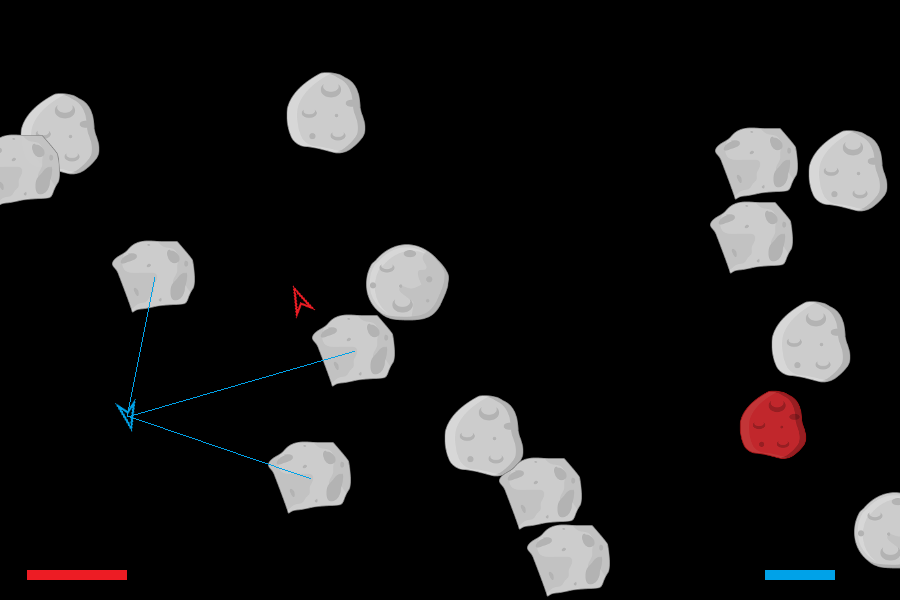
\includegraphics[width=145mm, height=100mm]{./Obrazky/N_nearest_asteroids.png}
\caption{Ukázka senzoru ``\emph{N} nejbližších asteroidů od vesmírné lodi'' pro \emph{N}=3}
\label{obr02:}
\end{figure}


\section{Akční plán}
Druhou zmíněnou abstrakcí jsou akční plány. Jejich cílem je podobně jako u senzoru pracovat namísto akcí nízké úrovně s akcemi vyšší úrovně. V případě akcí toto znamená namísto volby jednotlivých elementárních akcí volit akční plány, který mají komplexnější cíl.
Akční plán reprezentuje posloupnost elementárních akcí, které má agent vykonávat v následujících krocích hry.
Cíl akčního plánu se liší podle toho, o jaký druh se jedná.
\par
Podobně jako u senzorických metod i zde hledání většiny akčních plánů probíhá simulací hry.

\subsection{Jednotlivé plány}
\begin{itemize}
    \item Útočný plán - 
        Tento akční plán hledá posloupnost rotací následovaných střelou tak, aby byl sestřelen asteroid, který poté zasáhne nepřátelskou loď.        
        Simulace inkrementálně prochází všechny možné otočení a následné střely. Vesmírná loď se v rámci simulace otočí, vystřelí se střela a následně se sleduje, zda tato střela zasáhne libovolný velký nebo střední asteroid.
        Nad tímto asteroidem se následně zkouší, zda-li asteroidy vzniklé rozstřelením zasáhnou nepřátelskou loď. Rozstřelení asteroidu se zkouší pro oba typy střel.
        \par
        V případě nesestřelení žádného asteoridu, nebo minutí nepřátelské lodi rozstřeleným asteroidem, se v simulaci vesmírná loď pokusí provést další rotaci a celý pokus o střelbu opakovat.
        Pokud v simulaci nastalo úspěšné sestřelení, tak se vrací útočný akční plán, který obsahuje přílušný počet rotací následovaný střelou.
    
    \item Obranný plán - Pro hledání obraného plánu je nejprve potřeba vědět, před kterým asteroidem je potřeba vesmírnou loď bránit. 
        Zde využijeme připravené senzory. Posloupnost obraného plánu obsahuje dvě části. V první části se vesmírná loď rotuje tak, aby mířila na asteroid, před kterým je potřeba se bránit.
        A v druhé části probíhá samotná střelba, ta spočívá v jediné elementární akci střelby. Pro vyhodnocení, zda vystřelením střely sestřelíme konkrétní asteroid, využijeme připravené senzorické metody.
        \par
        Nalezení potřebné rotace pro nasměrování vesmírné lodi k nebezpečnému asteroidu probíhá statickým výpočtem bez použití simulace.
        Nejprve zjistíme přesnou polohu, kde k potenciální srážce dojde. V případě, že vesmírná loď, anebo asteroid stojí staticky na místě, tak ke srážce dojde na současné poloze vesmírné lodi.
        V případě pohybu obou objektů se poloha střetu nachází na průniku jejich trajektorií. Tuto polohu střetu musíme vzít v úvahu při nasměrovávání vesmírné rakety k asteroidu.        
        Pokud by se vesmírná loď otočila pouze vzhledem k současné poloze asteroidu, tak by vystřelením mohla letící asteroid minout.
        Proto namísto současné polohy asteroidu musí vesmírná loď mířit na cílovou polohu.
        Cílová poloha pro nás bude bod, který leží na úsečce spojující současnou polohu asteroidu a polohu střetu objektů a to ve vzdálenosti 15\% jejich vzdálenosti blíže k poloze asteroidu. 
        Tímto způsobem bude vesmírná loď mířit mírně před asteroid do jeho trajektorie. Empiricky jsem vyzkoušel, že tato vzdálenost v praxi funguje velmi dobře.
        Po vypočtení cílové polohy stačí spočítat rozdíl současného úhlu vesmírné lodi od úhlu směřujícímu k cílové poloze. A z tohoto rozdílu snadno získáme potřebný počet rotací. Ty budou tvořit výsledný obranný plán.
        
    
    \item Úhybný plán - Jedná se také o defenzivní plán, ale namísto přímého sestřelení nebezpečného asteroidu se tento akční plán snaží asteroidu vyhnout.
    Podobně jako u obranného plánu potřebujeme vědět, před jakým asteroidem je potřeba se vyhnout. Tento asteroid je stejně jako v předchozím obranném plánu získaný senzorem. Po nalezení nebezpečného asteroidu simulace postupně prochází všechny možné otočení a následnou akceleraci.
    Počet potřebných akcí akcelerace probíhá také inkrementálně. Nejprve se vyzkouší provedení jedné akce akcelerace a následně se simuluje pohyb vesmírné lodi a asteroidu bez dalšího akcelerování.
    Při srážce vesmírné lodi s asteroidem se oba objekty vrátí na původní místo a vyzkouší se o jednu akci akcelerace více než v předešlém případě.
    V případě úspěšného vyhnutí bude úhybný akční plán obsahovat posloupnost akcí rotace následované posloupností správného počtu akcí akcelerace.
    
    \item Zastavovací plán - Tento plán jsem vytvořil na základě sledování chování agenta využívajícího úhybný plán. Úhybný plán vždy vrací nejkratší možný plán, který stačí na vyhnutí se srážce. Jako důsledek proto obvykle plán obsahuje minimální počet rotací, který je dostačující.
        To mělo v praxi za následek, že agent, který se řídí pouze úhybným plánem používá akceleraci mnohem častěji než rotace a lítá proto obrovskou rychlostí přibližně stejným směrem napříč prostorem. Proto mě napadlo vytvořit akční plán, který vesmírnou loď uvede do klidu.
        \par
        Zastavovací plán má přímočarou myšlenku. 
        Nejdříve se vesmírná loď otočí tak, aby byla nasměrována proti směru svého pohybu a následně provede potřebný počet akcelerací, aby zpomalila až do úplného zastavení. 
        V tomto akčním plánu není potřeba provádět simulaci, výpočet potřebného počtu rotací i následných akcelerací lze spočítat statickým výpočtem.
        
        \par
        V kombinaci s úhybným plánem se agent chová v jistém smyslu klidněji.
        Namísto zběsilého letu napříč prostorem se vesmírná loď po vyhnutí asteroidu zastaví.            
        \par
        Tento akční plán jsem vytvořil na základě svého lidského instinktu, jak bych očekával od inteligentního agenta, že by se mohl chovat. Zda bude mít tento akční plán v praxi reálný přínos uvidíme v pozdější kapitole, kde budeme s akčními plány experimentovat.
        
        
\end{itemize}


\subsection{Přepočítávání akčních plánů}
Získávání akčních plánů je výpočetně náročné, proto jsem se pokusil jejich přepočítávání vhodně omezit. Akční plány nám vracejí posloupnost akcí na více kroků dopředu a proto není vždy potřeba je přepočítávat v každém kroku.
Změny mezi dvěmi po sobě jdoucími stavy hry nejsou veliké, ale mohou být občas dostatečné na to, aby se přepočítaný plán lišil od toho spočítaného v předchozím kroku.
V každém kroku hry se proto rozhoduje, zda se daný plán přepočítá, nebo se bude následovat plán původní. 
Plán se bude přepočítávat ve dvou možných případech, těmi jsou uplynutí daného počtu pasivních kroků, ve kterých jsme pouze pokračovali v již vytvořeném původním plánu, a nebo jeho dokončení.
Počet neaktivních kroků, po kterých dochází k přepočítávání plánu, se rovná konstaně \emph{\uppercase{inactive\_steps\_limit}}. 
S vyšším počtem pasivních kroků se velmi výrazně snižuje výpočetní čas potřebný k odehrání hry, ale počet kroků, který hra trvala, se sníží jen minimálně (viz \ref{obr03:}).
Je zde vidět, že kvalita hráčů se mírně snižuje, ale v porovnání kolik se ušetří výpočetního času, je tato ztráta kvality zanedbatelná.
V příštích kapitolách se nám bude pro učení agentů hodit odehrát velké množství her, proto si dovolíme nastavit vyšší počet pasivních kroků.


\begin{figure}[hp]

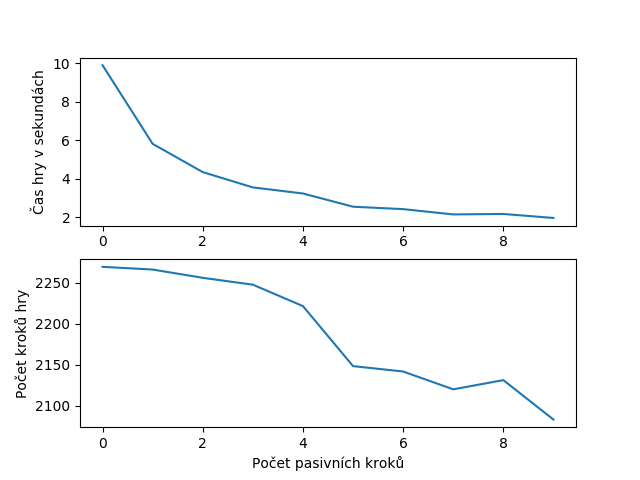
\includegraphics[width=145mm, height=120mm]{./Obrazky/Inactive_steps_comparison2.png}
\caption{Srovnání počtu neaktivních kroků k průměrné délce hry. Čísla byla získána průměrováním 40 her, kde proti sobě hráli agenti využívající pouze obranných plánů.}
\label{obr03:}
\end{figure}

\subsection{Použití akčních plánů}
Metody, které vypočítávají akční plán vracejí kromě plánů samotných i jejich délku. 
V případě nenalezení akčního plánu se místo jeho délky vrací konstanta \emph{\uppercase{not\_found\_steps\_count}} vysoké hodnoty, ta reprezentuje, že akční plán neexistuje.
Díky tomu lze tyto metody použít také jako senzorické metody. 




\chapter{Genetické programování}

\section{Základní princip}
Genetické programování je evoluční technika, která vytváří počítačové programy. Cílem genetického programování je vyřešit co nejlépe zadaný problém.
Nespecifikujeme jak je potřeba ho vyřešit, ale víme, co je potřeba vyřešit.
\par
Každý program budeme nazývat jedincem a množině jedinců budeme říkat populace. Algoritmus pak běží iterativně v generacích. 
V každé iteraci se provede výběr nějakých jedinců z populace, ti se pomocí genetických operátorů upraví a nakonec se rozhoduje, kteří z nich přežijí do další generace.
Populaci na začátku iterace nazýváme rodiče a populaci, která bylo nakonci iterace pro další generaci, nazýváme potomky.
Každý program představuje jedno řešení daného problému. Kvalitu tohoto řešení ohodnocujeme takzvanou fitness funkcí. Čím vyšší hodnotu této funkce jedinec získá, tím lépe řeší daný problém.
\subsection{Reprezentace}

Program je obvykle reprezentovaný syntaktickým stromem. Stromy ve vnitřních uzlech obsahují funkce (neterminály) a v listech terminály.
Vyhodnocení stromu probíhá od listů ke kořeni a výsledek programu je pak hodnota kořenu.

\subsection{Inicializace populace}
Na začátku evoluce potřebujeme inicializovat populaci. Na počátku jsou jedinci vytvořeni náhodně. Obvykle se k vytvoření jedinců používají dvě metody.
První z nich je vytváření jedinců s pevně danou hloubkou stromu, kde v listech jsou vždy už jen terminály. Druhou metodou je stavět strom náhodně z předem daného počtu neterminálů.
Po vyčerpání počtu neterminálů se již opět přidají terminály jako listy. Tato metoda vytváří jedince různých velikostí a tvarů.
Častou praxí je prvotní populaci vytvořit tak, že každá z metod vytvoří polovinu jedinců. 

\subsection{Selekce}
V každé iteraci chceme vybrat několik jedinců, nad kterými budeme provádět různé genetické operátory. Snahou je vybírat jedince s vyšší hodnotou fitness funkce.
Asi nejpoužívanější metodou selekce je turnajová selekce. Náhodně se zvolí daný počet jedinců, ti se porovnají mezi sebou na základě jejich hodnoty fitness funkce a nejlepší z nich je pak zvolen do výběru.
Dalším z mnoha metod selekce je ruletová selekce. Zde je pravděpodobnost zvolení jedince do výběru přímo úměrná jeho hodnotě fitness funkce.
Pravděpodobnost výběru i-tého jedince je 
\newline $p(i) = \frac{f(i)}{\sum_{j=1}^{n} f(j)} $. \newline
Ruletová selekce má jednoduchou implementaci a zároveň je rychlá na výpočet. 
Jejím problémem je ale předčasná konvergence k lokálnímu optimu.
\par
Genetické operátory mohou občas upravit nejlepšího jedince tak, že se jeho hodnota fitness funkce výrazně zhorší.
Z tohoto důvodu se často používá technika zvaná elitismus, která automaticky do další generace vybere několik nejlepších současných jedinců. 
Tímto způsobem máme zajištěno, že neztratíme nejlepší jedince.



\url{https://www.researchgate.net/publication/259461147_Selection_Methods_for_Genetic_Algorithms}

\subsection{Genetické operátory}
Genetické operátory jsou dvojího druhu, křížení a mutace. Myšlenkou křížení je vzít dva jedince, nazývejme je rodiče, a pomocí křížení informací každého z nich vytvořit nového potomka.
V genetickém programování pracujeme s jedinci reprezentovanými stromy, proto křížení jedinců představuje křížení jejich stromů. V každém z rodičů se zvolí jeden uzel. 
Výsledný potomek vypadá jako první rodič, jen na původním místě vybraného uzlu bude nyní podstrom, který je zavěšený pod vybraným uzlem druhého rodiče.
\par
Druhým genetickým operátorem je mutace, ta již nepotřebuje mít dva rodiče, ale úprava se provede nad jedincem samotným.
Mutovat můžeme v jedinci buď jediný bod, nebo celý nějaký podstrom. V případě mutace podstromu se namísto vybraného podstromu vygeneruje zcela nový podstrom. 
Toto v zásadě představuje křížení s novým náhodně vytvořeným jedincem.
\newline
Mutace jediného bodu změní náhodně jediný uzel ve stromě. V případě terminálu se může vybrat libovolný jiný terminál. A v případě vnitřního uzlu může být vybraný libovolný jiný neterminál, který je stejné arity.

\subsection{Typované x netypované}


\section{Využití}

\section{Aplikace}





\begin{figure}[p]\centering
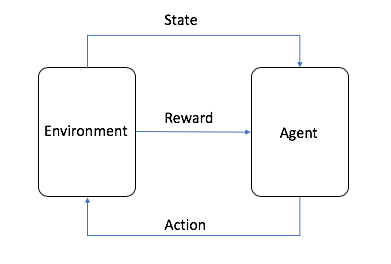
\includegraphics[width=140mm, height=140mm]{./agent_enviroment}
\caption{Herní cyklus}
\label{obr03:Nhust}
\end{figure}

\chapter{Hluboké Q-učení}

\section{Základní princip}
\subsection{Neuronová síť}

\subsection{Q-učení}
\subsection{Hluboké q-učení}

\section{Využití}
Kde se používá v praxi.


\section{Aplikace}
\subsection{Úvod}
Herní prostředí nám v každém kroku vrací odměnu, kterou oba z hráčů za jejich akci obdrželi. Tuto informaci jsme v experimentech provedených v rámci genetického programování, nevyužili, ale zde budou hrát velkou roli.
Za každý krok, kdy hra ještě neskončila získávají agenti automaticky odměnu 1. Na konci hry agent obdrží vysokou odměnu v případě výhry a v případě prohry naopak získá penalizaci v podobě odměnu vysoké záporné hodnoty. Tyto hodnoty se pro jednotlivé experimenty mírně liší.
Odměnu za výhru, nebo prohru získá agent až na úplném konci hry, to může ztěžovat učící proces. Proto prostředí dává agentům i průběžné menší odměny, pro lepší možnost učení se.

Konkrétně to jsou následující odměny:
\begin{itemize}
    \item Sestřelení asteroidu
        \newline
        Za každý sestřelený asteroid získává agent odměnu hodnoty 5.
    \item Zasažení asteroidem nepřátelské vesmírné lodi
        \newline
        Zranění nepřítele je právě to, co agent potřebuje pro přiblížění se vítězství, proto za každé takové zasažení získává od prostředí odměnu v hodnotě 20.
    \item Zasažení asteroidem vlastní vesmírné lodi
        \newline
        Takový stav je pro agenta znevýhodňující a cílem je se mu vyvarovat, proto za takovýto stav agent od prostředí dostává penalizaci v hodnotě -10.
\end{itemize}


\todo{presunout do kapitoly o deep q}
V rámci učení agentů budeme využívat epsilon-hladového (ang. epsilon-greedy) přístupu. V každém kroku q-učení volíme další akci a epsilon-hladový přístup nám v tom pomáhá následovně.
Vygenerujeme náhodnou hodnotou z intervalu $(0,1)$ a pokud je tato hodnota menší než hodnota epsilon, tak provedeme volbu akce náhodně, v opačném případě volíme nejlepší akce dle q-sítě.
Hodnota epsilon se na počátku inicializuje na hodnotu 1 a po každé zahrané hře se sníží vynásobením koeficientem menším než 1. 
Epsilon-hladový přístup způsobuje, že z počátku učení se zkoušejí náhodné akce a v průběhu přechází ze zkoušení nových akcí do prohledávání již osvědčených akcí.

\todo{presunout do kapitoly o deep q}
\par
V Hlubokém učení se chceme při trénování vyvarovat závislostí na předchozích stavech. K tomu využijeme konceptu přehrávání zkušeností (ang. Experience replay).
Při hraní hry si v každém kroku ukládáme do paměti pětici současného stavu, provedené akce, obdržené odměny, stavu, do kterého jsme se dostali a informace zda hra neskončila.
Po konci zahrání hry následně náhodně vybíráme tyto pětice z paměti a trénování provádíme na nich.






\subsection{Experiment 4: Soupeření s obranným agentem}
V 1. experimentu jsme za pomocí genetického programování hledali agenta, který je úspěšný v souboji s obranným jedincem. Pro určení jak agent v souboji obstál jsme využívali fitness funkci.
Zde, pomocí hlubokého q učení, budeme také učit agenta vzájemnými souboji s obranným agentem, ale budeme namísto fitness funkce používat pro trénování odměny.

S 1. experimentem zde bude také stejný přístup ke vstupům a výstupům. 
Na vstupu budou opět délky všech čtyř akčních plánů a počet kroků před srážkou vesmírné lodi s asteroidem.
A na výstupu čtyři hodnoty reprezentující výběr konkrétního akčního plánu.

Q učení spočívá v učení se rozhodování akcí. Akce zde v tomto pojetí však nebudou elementární akce, nýbrž akční plány. 
Q-síť bude tedy volit akční plány a proto zde budeme muset provádět mezikrok pro přechod od akčních plánů k akcím.
Nejprve vždy zvolíme akční plán a následně pro pokračování v simulaci hry z vybraného akčního plánu vybereme první akci.
V tomto experimentu budeme využívat přehrávání zkušeností, tj. budeme průběžně ukládat informace o přechodech do dalších stavů. 
I Zde, pro zapamatování si zkušenosti, platí, že akcí budeme rozumět akční plán.


Parametry experimentu:
\begin{itemize}
    \item Na konci hry agent obdrží agent odměnu v hodnotě 2000 v případě výhry a -1000 v případě prohry.
    \item Q-síť je hustá neuronová síť s pěti vstupy, čtyřmi výstupy a jednou skrytou vrstvou. 
    \item Během učení bude zahráno 1500 her.
    \item Konstanta pro snižování epsilon je nastavena na 0.998. To znamená, že například po zahrání 1400 her se bude v další hře volit akce náhodně jen v 6\% případů. 
\end{itemize}

\par
V souboji s obranným agentem se výslednému agentovi podařilo zvítězil pouze ve čtyřech hrách. 
Nepodařilo se nám tedy sice nalézt agenta, který by porážel obranného agenta, ale dosáhli jsme jiného zajímavého výsledku.
Velkým přínosem tohoto experimentu je pestrá strategie nalezeného agenta. Výsledný agent ve velkém zastoupení používá všechny akční plány (viz \ref{Výsledek experimentu 04}). 
Výsledkem je agent, který se brání nejen sestřelováním nepřátelskqých asteroidů, ale i vyhýbáním se. A díky tomu se agent také pohybuje a nezůstává staticky stát na stejném místě po celou dobu hry.
Toho se nám také podařilo dosáhnout ve 3. experimentu, ale srovnání s agentem získaným ze 3. experimentu je tento agent daleko více obranyschopný.




\begin{figure}[p]\centering
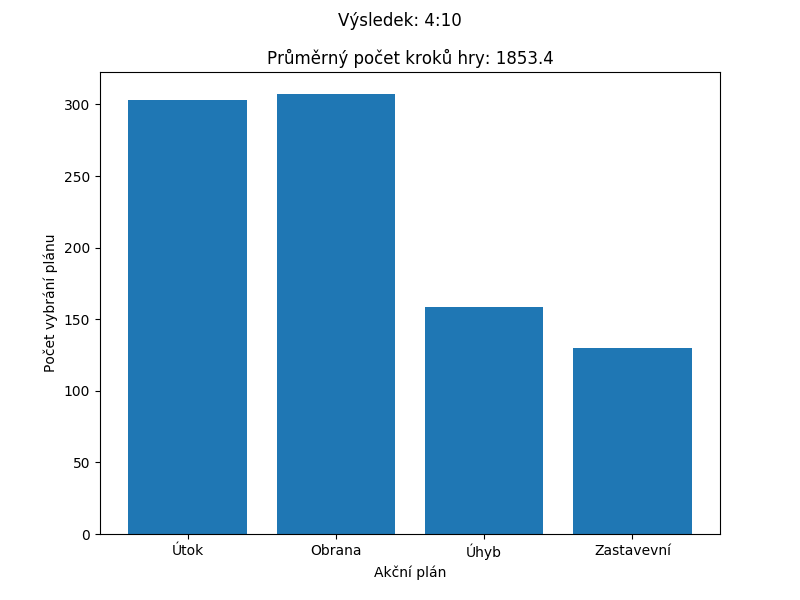
\includegraphics[width=145mm, height=110mm]{./Obrazky/Experiment04Results.png}
\caption{Výsledek experimentu 4}
\label{Výsledek experimentu 04}
\end{figure}

\subsection{Experiment 5: Soupeření s obranným agentem - Rozšířeno}
V předchozím experimentu jsme dosáhli zajímavého chování agenta, ale nepodařilo se nám stabilně vyhrávat nad obranným agentem.
Zkusíme proto předchozí experiment rozšířit. 
V tomto experimentu zkusíme přidat další vstupní argumenty, které by mohli agentovi pomoct v rozhodování.

Přidané parametry:
\begin{itemize}
    \item Dvojice počtu zbývajících životů obou agentů            
    \item Počet nebezepčných asteroidů v blízké vzdálenosti od agenta
    \item Celkový současný počet nebezpečných asteroidů v celé hře
\end{itemize}
Snaha všech přidaných argumentů je rozšířit agentovi poznání o současném stavu hry a díky tomu dát agentovi možnost se komplexněji rozhodovat pro akční plány.

Parametry experimentu:
\begin{itemize}
    \item Odměny za finální stav hry zůstávají stejné. Na konci hry agent obdrží agent odměnu v hodnotě 2000 v případě výhry a -1000 v případě prohry.
    \item Q-síť je stejná síť jako v předchozím případě, jen namísto pěti vstupních argumentů, bude nyní přijímat vstupů devět.
    \item V tomto experimentu zkusíme kvůli rozšíření vstupních argumentů také prodloužit trénování sítě, proto bude v rámci trénování zahráno 3000 her.
    \item Adekvátně ke zvýšení počtu zahraných her také zvětšíme konstantu pro snižování epsilon z hodnoty 0.998 na 0.9989. Díky tomu bude stejné pravděpodobnosti 6\% pro volbu náhodné akce dosaženo přibližně po zahrání 2550 her.
\end{itemize}

\begin{figure}[p]\centering
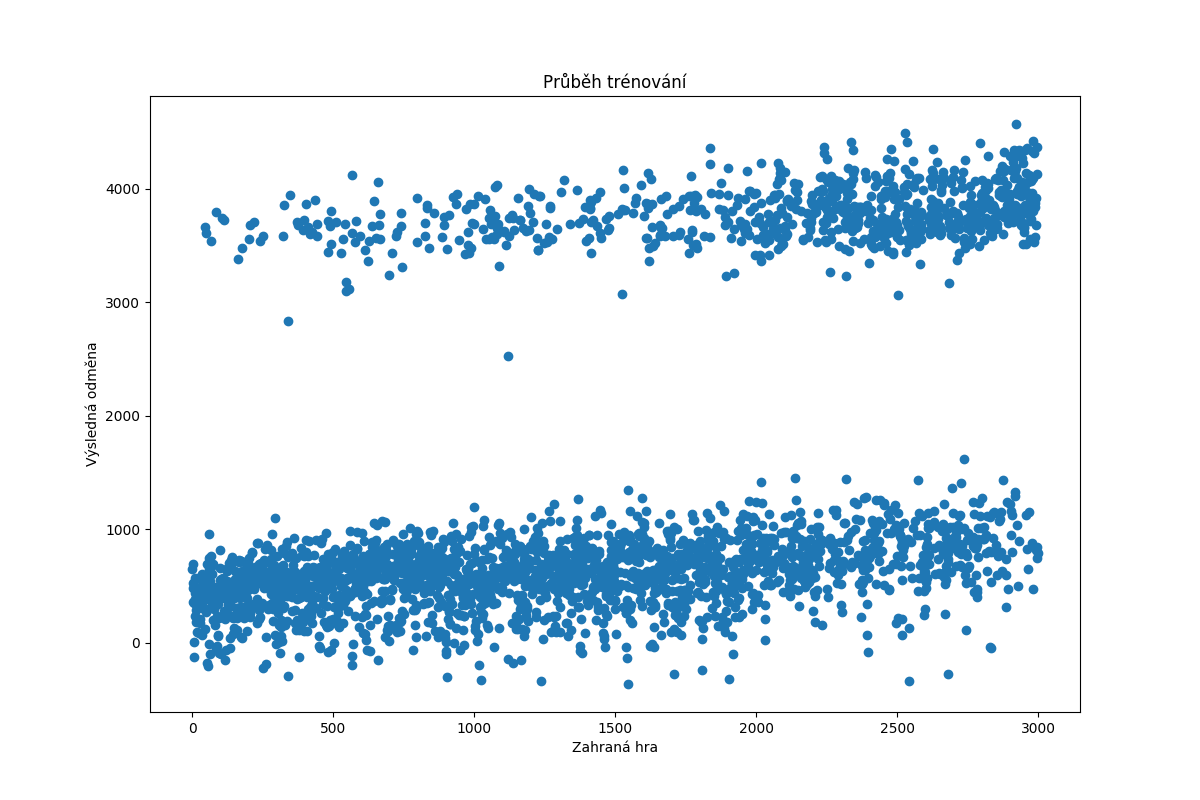
\includegraphics[width=145mm, height=110mm]{./Obrazky/Experiment05Training.png}
\caption{Průběh trénování v experimentu 5 - Výsledné odměny jsou součtem počtu kroků hry a odměny (resp. penalizace) za výhru (resp. prohru). Samotné tyto odměny tvoří rozdíl v hodnotě 3000, díky tomu je z obrázku zřetelné, ve kterých hrách agent vyhrál.}
\label{Průběh trénování experimentu 06}
\end{figure}




\begin{figure}[p]\centering
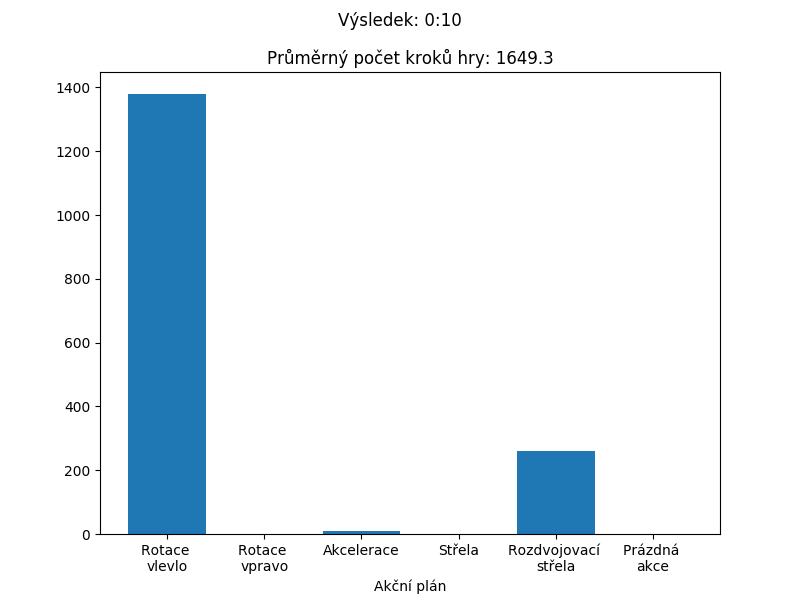
\includegraphics[width=145mm, height=110mm]{./Obrazky/Experiment05Results.png}
\caption{Výsledek experimentu 5}
\label{Průběh trénování experimentu 06}
\end{figure}


Výsledný agent dopadlo velmi úspěšně. Z průběhu trénování vidíme, že agent se velmi dobře učil a od přibližně 2300. hry (viz \ref{Průběh trénování experimentu 06}) už začal vyhrávat ve větší části her.
Rozšířením vstupních argumentů a přidání trénovacích her se nám podařilo zlepšit výsledek z předchozícho experimentu.
Agent sice ztratil pestrost akčních plánů, ale za to se významně zlepšil ve vyhrávání. Z výsledku 4:10 z předchozícho experimentu se zlepšil na 10:3.
Zajímavé na nalezeném agentovi je také jeho agresivita. Agent používá útočný akční plán přibližně dvakrát tak často jako obranný plán.

Při testování výsledného agenta jsem si všimnul, že zahrání jedné hry je časově značně náročné, přičemž to co při simulaci trvalo netriviální objem času bylo samotné dotazování q-sítě na akční plán.
Při snaze tento problém vyřešit jsem zjistil, že v některých stavech hry jsou všechny akční plány prázdné. 
Toto může nastat v případě kdy agent stojí na místě, není ohrožený žádným asteroidem a zároveň nenalezl žádný asteroid, kterým by mohl přímo ohrozit nepřítele.
V takovém stavu nemá velký smysl rozhodovat o volbě konkrétního akčního plánu. Proto jsem nastavil, že v takových případech agent rozhodování provádět nebude.

Podobně jsem také vypozoroval, že během jedné hry často nastane situaci, že právě jeden z akčních plánů je neprázdný. Překvapením pro mě bylo, že q-síť v takovém případě někdy volila jiný prázdný plán před tímto.
Proto jsem nastavil vyjímku i pro tyto případy a v současnou chvíli platí, že když agent má k dispozici právě jeden neprázdný akční plán, tak ho volí automaticky bez dotazování se q-sítě.
Těmito opatřeními bylo dosaženo lepší časové náročnosti hraní hry a také byl agent v souboji úspěšnější. Zlepšení agenta si vysvětluji právě tím, že volba jakéhokoliv neprázdného plánu před prázdným je vždy výhodnější.


\todo{Dokončit 7.Experiment}\newline
\todo{Kapitola o Deep q}\newline
\todo{Transponovat kapitoly o algoritmech a experimentech}\newline
\todo{Naprogramovat spouštění experimentů}\newline
\todo{Popsat spouštění agentů}\newline






\subsection{Experiment 6: Elementární agent proti obrannému agentovi}
V tomto experimentu zkusíme sestoupit od abstrakcí v podobě akčních plánů k elementárním akcím.
Tentokrát nebudeme q-síť používat k volbě akčního plánu, ale přímo k volbě elementární akce.
Výsledný agent bude volit vždy jen jednu akci, proto nebudeme moci využít koncept přepočítávání akčních plánů a agent se bude muset rozhodovat v každém kroku.
Opět budeme k trénování využívat soubojů s obranným agentem a učit se na základě odměn získaných od herního prostředí.

\par
K pěti elementárním akcím, pro které se bude agent rozhodovat, přidáme navíc také možnost prázdné akce. 
Nebudeme zde volit akční plány, proto tedy ani nemá dobrý smysl používat jejich délky jako argumenty pro rozhodování. Proto zde můžeme zvolit zcela jiný přístup.
Samotné simulace pro získání akčních plánů jsou výpočetně velmi náročné, a tedy díky tomu, že zde volíme jednodušší přístup, tak budeme schopni, oproti předchozím experimentům, zahrát v rámci trénování větší množství her.

\par
Jako vstupní argumenty jsem zvolil následující hodnoty:
\begin{itemize}
    \item Vektor současného pohybu vesmírné lodi
    \item Úhel natočení vesmírné lodi
    \item Počet uplynulých kroků od posledního výstřelu
    \item Relativní poloha nepřátelské lodi
    \item Relativní polohy tří nejbližších nebezpečných asteroidů
\end{itemize}

Parametry experimentu:
\begin{itemize}
    \item \todo{sjednotit odmeny a penalizaci}
    \item Q-síť je hustá neuronová síť s dvěmi skrytými vstvami, čtrnácti vstupními a šesti výstupními hodnotami.
    \item Díky nevyužívání akčních plánů bude hraní her rychlejší, proto pro trénování zahrajeme 10000 her.
    \item Konstanta pro snižoání epsilon je nastavena na hodnotu \todo{0.9998}
    \item V posledních 5\% her se nebude epsilon-hladový přístup používat a budou se volit nejlepší známé akce.
\end{itemize}


Výsledný agent proti obrannému agentovi nedopadl úspěšně. V souboji byl jednoznačně poražen se skóre 0:10.
A z přehledu používaných akcí během souboje můžeme i vypozorovat proč takto dopadl. Z elementárních operací se rozhodoval v drtivé většině pro rotaci vlevo a rozdvojovací střelu.
To v praxi znamená, že se agent naučil točit dokola a kdykoliv může, tak vystřelit. Tato strategie skutečně přináší nějaké výsledky.
Touto kombinací rotace a střelby se agent dokáže ubránit před srážkou s některými asteroidy, které by ho jinak zasáhly. Zároveň tímto způsobem sestřeluje netriviální množství asteroidů, které se kolem něho nacházejí a tím potenciálně staví nepřítele do ohrožení.
Avšak pro toto chování se agent rozhoduje bezmyšlenkovitě. 
Nemíří na žádné konkrétní asteroidy, ani na nepřátelskou loď.
Největší slabinou je, že agent se zde prakticky vůbec nenaučil bránit.
Veškeré asteroidy, před kterými se agent ubrání, zasáhne vesměs náhodně.


\begin{figure}[p]\centering
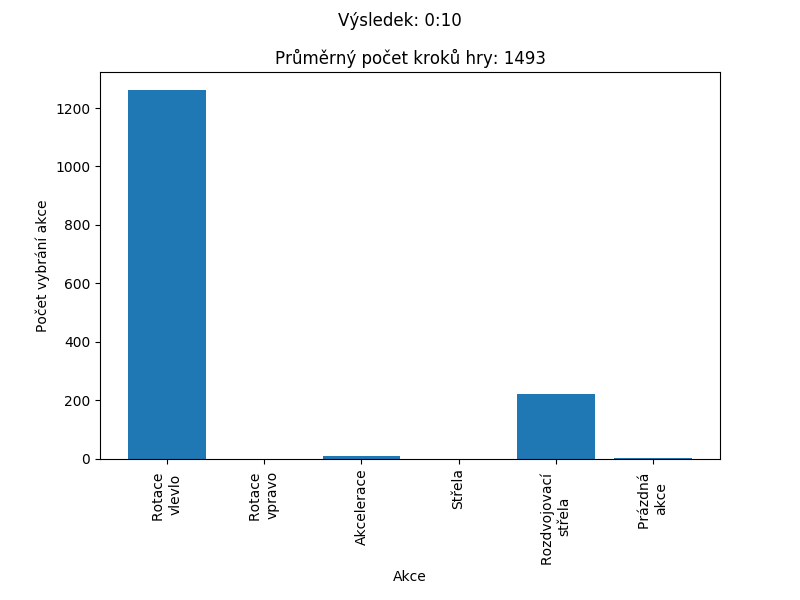
\includegraphics[width=145mm, height=110mm]{./Obrazky/Experiment06Results.png}
\caption{Výsledek experimentu 6}
\label{Výsledek experimentu 06}
\end{figure}
    



\subsection{Experiment 7: Dva elementární agenti}
Tento experiment rozšiřuje experiment předchozí. Budeme opět pracovat s elementárním agentem reprezentovaného neuronovou sítí stejného formátu jako v předhozím případě.
Tentokrát ale nebudeme při trénování hrát hry proti obrannému agentovi, nýbrž proti dalšímu elementárnímu agentovi, který bude také zároveň trénován.
Budeme tedy provádět dvojí q-učení simultánně. Teoreticky bychom měli dosáhnout vzájemného adaptivního učení, kde se každý z agentů snaží zlepšovat proti svému nepříteli a postupně se tak budou oba zlepšovat.
\par


Parametry experimentu:
\begin{itemize}
    \item \todo{sjednotit odmeny a penalizaci}
    \item Každý agent bude reprezentován vlastní q-sítí stejného formátu jako v předchozím experimentu.
    \item Tím, že pro souboj nebudeme používat obranného agenta, ale dalšího elementárního agenta, ušetříme čas na výpočtu obranného agenta. V rámci trénování tedy zahrajeme 20000 her.  
    \item Konstanta pro snižoání epsilon je nastavena na hodnotu 0.9998
    \item V posledních 5\% her se nebude epsilon-hladový přístup používat a budou se volit nejlepší známé akce.
\end{itemize}


\begin{figure}[p]\centering
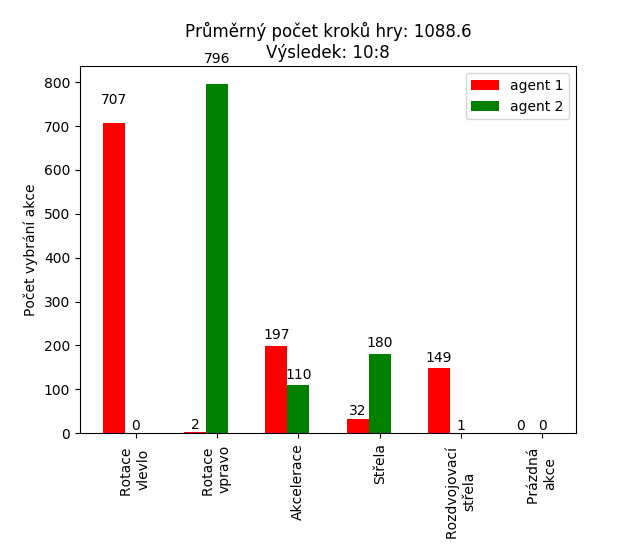
\includegraphics[width=145mm, height=110mm]{./Obrazky/Experiment07Results.png}
\caption{Výsledek experimentu 7}
\label{Výsledek experimentu 07}
\end{figure}
        
% 
\chapter{NEAT}

\section{Základní princip}

\section{Využití}
Kde se používá v praxi.


\section{Aplikace}
Jak jsem to použil já a jakých výsledků jsem dosáhl.




\chapter*{Závěr}
V této práci se nám úspěšně podařilo vymyslet a naimplementovat abstrakce v podobě senzorů a akčních plánů do vytvořené vesmírné hry.
Tyto abstrakce umožnili zrychlení výpočtu her a také dali agentům nástroj jak se lépe v prostředí orientovat a jak na něj vhodně reagovat.
Dále jsme se seznámili s algoritmy genetického programování a hlubokého Q-učení.
Z cílů, které jsme si v úvodu stanovili, byli tedy kompletně splněny první tři.

V závěrečné části práce jsme zmíněné algoritmy aplikovali v našem herním prostředí a provedli s nimi sérii experimentů.
V rámci nich jsme nalezli agenty, kteří se naučili bránit a útočit dostatečně dobře na to, aby pro člověka bylo téměř nemožné je porazit.
Tedy cíl nalézt agenty, kteří budou naši hru hrát velmi dobře, byl také splněn.

Bohužel se nám nepodařilo nalézt agenty, kteří by byli dobří v pohybování se po herním prostoru a to ať už za záměrem úhybného manévru, nebo z důvodu získání lepší strategické pozice.
Jako důsledek se proto agenti chovají nepřirozeně staticky a pro člověka není příliš zábavné s nimi hrát.
Proto musíme konstatovat, že cíl nalézt agenty s pestrým chováním, splněn zcela nebyl.

V případě pokračování na této práci by stálo za to zamyslet se nad dalšími možnými akčními plány, obzvláště nad těmi, které by zlepšovaly pohyb vesmírné lodi po herním prostoru.
Hra může být také do budoucna lehce rozšiřitelná o další implementace agentů. Pro přidání dalšího agenta stačí implementovat jednoduchou metodu, která dostává stav hry a vrací akci a agent může být jednoduše do hry přidán. 

Kromě rozšiřování akčních plánů a přidávání dalších agentů by také mohlo být zajímavé prozkoumat další algoritmy umělé inteligence a vyzkoušet v rámci nich podobné přístupy, které byly použity v našich experimentech.

\addcontentsline{toc}{chapter}{Závěr}


%%% Seznam použité literatury
 %%% Seznam použité literatury (bibliografie)
%%%
%%% Pro vytváření bibliografie používáme bibTeX. Ten zpracovává
%%% citace v textu (např. makro \cite{...}) a vyhledává k nim literaturu
%%% v souboru literatura.bib.
%%%
%%% Příkaz \bibliographystyle určuje, jakým stylem budou citovány odkazy
%%% v textu. V závorce je název zvoleného souboru .bst. Styly plainnat
%%% a unsrt jsou standardní součástí latexových distribucí. Styl czplainnat
%%% je dodáván s touto šablonou a bibTeX ho hledá v aktuálním adresáři.

\bibliographystyle{czplainnat}    %% Autor (rok) s českými spojkami
% \bibliographystyle{plainnat}    %% Autor (rok) s anglickými spojkami
% \bibliographystyle{unsrt}       %% [číslo]

\renewcommand{\bibname}{Seznam použité literatury}

%%% Vytvoření seznamu literatury. Pozor, pokud jste necitovali ani jednu
%%% položku, seznam se automaticky vynechá.

\bibliography{literatura}

%%% Kdybyste chtěli bibliografii vytvářet ručně (bez bibTeXu), lze to udělat
%%% následovně. V takovém případě se řiďte normou ISO 690 a zvyklostmi v oboru.

% \begin{thebibliography}{99}
%
% \bibitem{lamport94}
%   {\sc Lamport,} Leslie.
%   \emph{\LaTeX: A Document Preparation System}.
%   2. vydání.
%   Massachusetts: Addison Wesley, 1994.
%   ISBN 0-201-52983-1.
%
% \end{thebibliography}


%%% Obrázky v bakalářské práci
%%% (pokud jich je malé množství, obvykle není třeba seznam uvádět)
\listoffigures

%%% Tabulky v bakalářské práci (opět nemusí být nutné uvádět)
%%% U matematických prací může být lepší přemístit seznam tabulek na začátek práce.
% \listoftables

%%% Použité zkratky v bakalářské práci (opět nemusí být nutné uvádět)
%%% U matematických prací může být lepší přemístit seznam zkratek na začátek práce.
% \chapwithtoc{Seznam použitých zkratek}

\appendix
% \chapter{Přílohy}

% \section{První příloha}

\openright
\end{document}
